\section{分布积分的极限}
\label{sec:weak-integral-limits}

弱收敛控制的是有界连续函数的期望。可是最常用的量，均值、方差、高阶矩，都是无界函数的期望。设$X_n\xrightarrow{\mathrm{d}}X$，$g$连续而无界，$\mathbb{E}[g(X_n)]$是否趋于$\mathbb{E}[g(X)]$？

第~\ref{sec:weak-mass-control}节的例子给出否定的回答。$X_n$以概率$1/n$取$n$、否则取$0$。对$f\in C_b$，$\mathbb{E}[f(X_n)]=(1-1/n)f(0)+f(n)/n\to f(0)$，所以$X_n\xrightarrow{\mathrm{d}}0$。可是
\[
 \mathbb{E}[X_n]=n\cdot\frac1n=1\quad\text{对一切}n,\qquad\mathbb{E}[0]=0 .
\]
远处那份越来越轻的质量，乘以越来越大的位置，始终贡献$1$。弱收敛看不到它，因为有界函数在远处的读数被$\sup\lvert f\rvert/n$压住了；期望却要乘以位置本身。每个$X_n$的各阶矩都有限，$\mathbb{E}[X_n^{k}]=n^{k-1}$，但这对极限毫无帮助。

\paragraph{一致可积条件}
补上的条件正是第~\ref{sec:weak-mass-control}节对比过的一致可积：要求远处质量乘以位置之后，对所有$n$一致地小。

\begin{theorem}[期望的收敛]
\label{thm:weak-ui-expectation}
设$\bm{X}_n\xrightarrow{\mathrm{d}}\bm{X}$，$g:\mathbb{R}^{d}\to\mathbb{R}$可测，$\mathbb{P}(\bm{X}\in D_g)=0$，并且$\{g(\bm{X}_n)\}$一致可积：
\begin{equation}
 \lim_{r\to\infty}\sup_{n}\mathbb{E}\bigl[\lvert g(\bm{X}_n)\rvert\,\mathbf{1}_{\{\lvert g(\bm{X}_n)\rvert>r\}}\bigr]=0 .
 \label{eq:weak-ui}
\end{equation}
则$\mathbb{E}[\lvert g(\bm{X})\rvert]<\infty$，并且
\begin{equation}
 \lim_{n\to\infty}\mathbb{E}\bigl[g(\bm{X}_n)\bigr]=\mathbb{E}\bigl[g(\bm{X})\bigr] .
 \label{eq:weak-ui-expectation}
\end{equation}
\end{theorem}

\begin{proof}
记$Y_n=g(\bm{X}_n)$，$Y=g(\bm{X})$。由连续映射定理，$Y_n\xrightarrow{\mathrm{d}}Y$，于是问题化为实随机变量。对$r>0$，令截断函数
\[
 h_r(y)=\max\bigl(-r,\min(y,r)\bigr) ,
\]
它有界连续，与$y$只在$\lvert y\rvert>r$处不同，并且在那里与$y$之差的绝对值不超过$\lvert y\rvert$。

先证$Y$可积。$y\mapsto\min(\lvert y\rvert,r)$有界连续，所以
\[
 \mathbb{E}\bigl[\min(\lvert Y\rvert,r)\bigr]=\lim_{n\to\infty}\mathbb{E}\bigl[\min(\lvert Y_n\rvert,r)\bigr]\leq\sup_{n}\mathbb{E}\bigl[\lvert Y_n\rvert\bigr] .
\]
由式~\eqref{eq:weak-ui}，取$r_0$使尾部积分不超过$1$，则$\mathbb{E}[\lvert Y_n\rvert]\leq r_0+1$，右边有限。令$r\to\infty$，由单调收敛定理，$\mathbb{E}[\lvert Y\rvert]\leq r_0+1<\infty$。

再拆三项。对每个$r$，
\[
 \begin{aligned}
 \bigl\lvert\mathbb{E}[Y_n]-\mathbb{E}[Y]\bigr\rvert
 &\leq\mathbb{E}\bigl[\lvert Y_n\rvert\mathbf{1}_{\{\lvert Y_n\rvert>r\}}\bigr]+\bigl\lvert\mathbb{E}[h_r(Y_n)]-\mathbb{E}[h_r(Y)]\bigr\rvert\\
 &\quad+\mathbb{E}\bigl[\lvert Y\rvert\mathbf{1}_{\{\lvert Y\rvert>r\}}\bigr] .
 \end{aligned}
\]
任取$\varepsilon>0$。由式~\eqref{eq:weak-ui}，取$r$使第一项对一切$n$不超过$\varepsilon$；$Y$可积，由支配收敛定理，$r$足够大时第三项也不超过$\varepsilon$。固定这个$r$，令$n\to\infty$，第二项趋于零。于是左边的上极限不超过$2\varepsilon$。
\end{proof}

证明中“先证可积”这一步本身给出一个不需要一致可积的结论：只要$Y_n\xrightarrow{\mathrm{d}}Y$，就有
\begin{equation}
 \mathbb{E}\bigl[\lvert Y\rvert\bigr]\leq\liminf_{n\to\infty}\mathbb{E}\bigl[\lvert Y_n\rvert\bigr] .
 \label{eq:weak-fatou}
\end{equation}
推导时把$\sup_n$换成$\liminf_n$即可。它是Fatou引理在依分布收敛下的形式：极限只可能丢失期望，不会凭空增加。开头的例子中，$\mathbb{E}[X_n]=1$，极限的期望$0$严格变小，丢失的正是逃到远处的那一份。

一致可积常用矩条件验证。若存在$\delta>0$与常数$C$，使$\mathbb{E}[\lvert Y_n\rvert^{1+\delta}]\leq C$对一切$n$成立，则由于在$\lvert y\rvert>r$处$(\lvert y\rvert/r)^{\delta}>1$，
\[
 \sup_n\mathbb{E}\bigl[\lvert Y_n\rvert\mathbf{1}_{\{\lvert Y_n\rvert>r\}}\bigr]\leq\frac{C}{r^{\delta}}\longrightarrow0 .
\]
注意要的是比一阶稍高的矩的一致界；开头的例子中，每个$X_n$的高阶矩虽然有限，却没有一致界。

\paragraph{二项分布的矩}
$X_n\sim\operatorname{Bin}(n,2/n)\xrightarrow{\mathrm{d}}N\sim\operatorname{Poisson}(2)$。二阶矩是否收敛？可以直接计算：
\[
 \mathbb{E}[X_n^{2}]=\operatorname{Var}(X_n)+(\mathbb{E}[X_n])^{2}=2\Bigl(1-\frac2n\Bigr)+4=6-\frac4n\longrightarrow6=\mathbb{E}[N^{2}] .
\]
用定理~\ref{thm:weak-ui-expectation}也能得到，并且不需要精确的公式，只要一个三阶矩的界。

$X_n(X_n-1)(X_n-2)$等于从成功的试验中按顺序取出三个不同试验的方式数，每个有序三元组全部成功的概率为$p^{3}$，这里$p=2/n$，所以
\[
 \mathbb{E}[X_n(X_n-1)(X_n-2)]=n(n-1)(n-2)p^{3}\leq(np)^{3}=8 .
\]
同理$\mathbb{E}[X_n(X_n-1)]\leq(np)^{2}=4$。由$x^{3}=x(x-1)(x-2)+3x(x-1)+x$，
\[
 \mathbb{E}[X_n^{3}]\leq8+3\cdot4+2=22 .
\]
取$Y_n=X_n^{2}$，$\delta=1/2$，$\sup_n\mathbb{E}[\lvert Y_n\rvert^{3/2}]\leq22$，所以$\{X_n^{2}\}$一致可积，$\mathbb{E}[X_n^{2}]\to\mathbb{E}[N^{2}]$。同样的论证对任意阶矩都适用。图~\ref{fig:weak-ui-truncation}把这个例子与开头的反例并列。

\begin{BookInlineFigure}
 \centering
 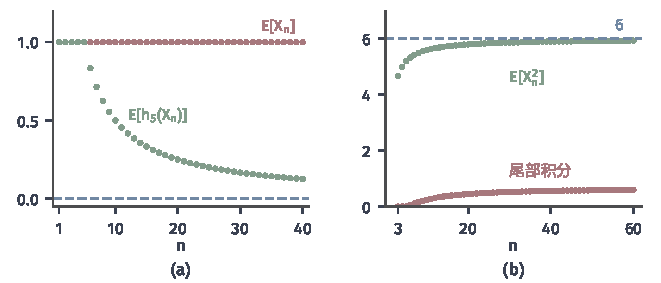
\includegraphics[width=112mm]{figures/07-probability/03-probability-limits/matplotlib/weak-ui-truncation/figure.pdf}
 \caption{期望能否随分布取极限。(a)$X_n$以概率$1/n$取$n$：$\mathbb{E}[X_n]$（红）恒为$1$，截断期望$\mathbb{E}[h_5(X_n)]$（绿）趋于极限的期望$0$（蓝色虚线），二者之差是$r=5$以外的尾部积分。(b)$X_n\sim\operatorname{Bin}(n,2/n)$：$\mathbb{E}[X_n^2]$（绿）趋于$6$（蓝色虚线），尾部积分$\mathbb{E}[X_n^2\mathbf{1}_{\{X_n^2>25\}}]$（红）对一切$n$都小于$0.7$，不随$n$增长。}
 \label{fig:weak-ui-truncation}
\end{BookInlineFigure}

\paragraph{与\texorpdfstring{$L^{1}$}{L1}收敛判据的区别}
第~\ref{chap:random-variable-convergence}章在同一概率空间上证明过：$X_n\xrightarrow{\mathbb{P}}X$且$\{X_n\}$一致可积，当且仅当$X_n\xrightarrow{L^{1}}X$，即$\mathbb{E}[\lvert X_n-X\rvert]\to0$。定理~\ref{thm:weak-ui-expectation}用的也是一致可积，但结论弱得多：它只说期望这一个数收敛，不涉及$\lvert X_n-X\rvert$，这个差可能根本没有定义。第~\ref{sec:weak-test-functions}节中$X(\omega)=\omega$、$X_n(\omega)=1-\omega$的例子里，期望恒等，而$\lvert1-2\omega\rvert$的平均$\mathbb{E}[\lvert X_n-X\rvert]=1/2$不趋于零。

\paragraph{不是期望的量}
定理处理的是固定函数$g$的期望。有些量由整个质量表或密度计算，不能写成某个固定$g$的期望，例如第~\ref{chap:information-measures}章的熵；弱收敛对它们没有一般的保证。格点均匀分布就是一例：$U_n$的质量表是$n$个$1/n$，任何只依赖各点质量大小的量都与$\operatorname{Unif}(0,1)$的密度无从比较，尽管$U_n\xrightarrow{\mathrm{d}}\operatorname{Unif}(0,1)$。这类量的极限要在相应的章节里另加条件讨论。
